% -*- coding: utf-8 -*-

\chapter{绪论}

\section{研究背景及意义}

随着云计算的爆发式增长，现代数据中心已演变为重要的信息基础设施。一个典型的大型数据中心可部署数十万台服务器，通过网卡、交换机、路由器和光纤线缆逐级互联，构成大规模数据中心网络（Data Center Network, DCN）。在此类物理基础设施之上，运行着种类繁多的大规模分布式系统——从搜索集群\upcite{barroso_web_search_2003}、分布式文件系统\upcite{ghemawat_google_file_2003}、云存储\upcite{calder_windows_azure_2011}，到分布式计算框架\upcite{dean_mapreduce_2004}，这些服务均依赖数据中心网络。在这类环境中，软硬件故障不可避免。当上层业务出现延迟飙升或连接中断时，数据中心网络的运维团队面临的第一个问题是：故障根源是否在网络侧？

Pingmesh系统\upcite{guo_pingmesh_2015}为这个问题给出了明确回答。其运维经验表明，约50\%被报告为“网络故障”的事件实际上并非由网络引起。Pingmesh利用数据中心内所有服务器作为探测节点，在机架内、ToR间和跨数据中心三个层级构建完全图式的TCP/HTTP Ping探测网络，每日产生超过2000亿次探测，覆盖了任意两台服务器之间的端到端延迟和丢包率。因此，如果Pingmesh数据未显示网络异常，则该故障事件几乎不可能由网络引起。换言之，Pingmesh告警是数据中心网络故障的可靠信号，当一个Pingmesh告警产生时，网络中必然存在需要立即处理的物理层问题。

然而，Pingmesh能够准确报告网络是否出了故障，却无法定位故障出在哪台设备。这一粒度缺陷的根源在于数据中心网络的架构特性：在Spine-Leaf拓扑中，多条等价路径通过ECMP（equal cost multipath，等价多路径路由）实现负载均衡。ECMP使用TCP/UDP五元组的哈希值来选择下一跳，因此即便服务器端知晓连接的五元组，也完全无法确定该连接在网络上实际穿越了哪条物理路径。Pingmesh的输出仅是一组粗粒度的异常端到端路径集合，所以数据中心网络的运维团队面临着第二个问题：真正的故障源头是哪个设备？

然而在解决第二个问题的同时，情况往往会进一步恶化。数据中心网络拓扑具有高度连通性，单一设备故障（如Spine交换机端口异常）会沿物理链路迅速蔓延，触发级联放大效应\upcite{yang_skynet_2025}。在这一过程中，部署于网络各层级的监控系统（从底层硬件传感器、网络协议守护进程到上层端到端探测）几乎同时被激活，在数十秒内产生海量关联告警，形成“告警风暴（Alert Storm）”\upcite{wang_2025_cola}。这些告警表面上杂乱无章，实则由同一个根因事件触发，沿拓扑路径逐级传播\upcite{yuan_neteventcause_2025}。告警风暴带来的直接后果是：原本就已因ECMP而模糊的故障位置信息，被数以千计的次生告警进一步淹没。运维人员面对的问题不仅仅是“从哪条路径找故障设备”，还有“从数千条告警中辨识出哪一条指向根因”。

针对上述问题，学术界与工业界已从多个技术维度提出了根因定位方法。在故障感知层面，以Pingmesh\upcite{guo_pingmesh_2015}为代表的主动探测系统通过端到端探测实现了网络级异常检测（其工作机制与部署优势详见第二章）。在根因定位层面，现有方法可大致归为三条技术路径：其一是将探测数据与网络拓扑相结合，利用物理连通性作为确定性约束推断故障位置\upcite{peng_detector_2017}\upcite{qian_ddrops_2022}\upcite{wang_hawkeye_2025}；其二是从历史告警数据中挖掘因果结构或关联规则\upcite{yuan_neteventcause_2025}\upcite{li_practical_2021}\upcite{zhao_2022_intelligentalarm}\upcite{huang_2024_5granalysis}；其三是借助大语言模型的语义理解能力对告警日志、设备配置和运维经验进行综合分析\upcite{wang_towards_2025}\upcite{zhang_tamofine-grained_2025}\upcite{huangjinchao_2024_largesmallmodel}。

上述方法各有侧重与局限。Pingmesh提供了可靠的故障感知信号，却因ECMP机制无法直接锚定物理根因设备；基于拓扑与探测的定位方法依赖路径与链路的精确对应，在ECMP多路径场景中精度受限；统计方法挖掘历史模式有效，但对未见过的故障类型泛化不足；LLM方法具备语义推理优势，却在多跳拓扑传播中缺乏空间感知能力。本文在综合对以上研究的洞察，提出一种结合主动探测触发、图算法剪枝与大语言模型推理的自动化网络根因定位方案。

\section{国内外研究现状}

在大规模数据中心网络中，网络故障的快速定位是保障服务可用性的核心运维任务。当网络中某个交换机、链路或光模块发生异常时，故障会沿物理拓扑和协议依赖关系向上下游传播，在短时间内触发大量关联告警。如何在大量告警中辨识因果关系、锁定初始故障源，是近年来学术界与工业界共同关注的研究问题。围绕这一目标，现有工作可从以下三个维度加以梳理：基于探测数据与网络拓扑的故障定位方法、基于统计与因果推断的根因定位方法、以及借助大语言模型进行语义推理的根因定位方法。

\subsection{基于探测数据与网络拓扑的故障定位方法}

一部分研究将探测数据与网络拓扑信息相结合，利用物理连通性作为确定性约束来推断故障的具体位置。这类方法的特点是：不依赖历史故障模式的学习，而是直接从拓扑结构和探测结果的几何关系或布尔关系中计算出故障位置。

\textbf{基于探测路径的故障链路推断。}deTector\upcite{peng_detector_2017}将探测路径的设计与网络拓扑显式结合，通过构造全覆盖的探针矩阵，使系统能够根据多条相交路径的丢包结果，利用布尔推断定位故障链路。其核心思想是：若一条端到端探测路径发生丢包，则故障必然位于该路径所经过的某条链路上；当多条异常路径在拓扑中相交时，交点即为最可疑的故障位置。然而在ECMP多路径环境下，探测路径与物理链路的对应关系并非一一映射，布尔推断的精度受限于探针矩阵对拓扑的覆盖完备性。

\textbf{基于数据平面遥测的丢包定位。}dDrops\upcite{qian_ddrops_2022}利用可编程数据平面在交换机的入口和出口流水线中嵌入轻量级状态机，通过上下游交换机协同比对数据包的到达与离开事件来判定丢包是否发生以及发生在哪一跳。Canary\upcite{chen_canary_2026}则采取了部分流量监控策略，仅追踪少量大流即可实现对全网络路径的覆盖，并利用Bloom Filter将路径信息编码到数据包头部以支持故障链路推断。

\textbf{基于遥测溯源的RDMA网络根因诊断。}Hawkeye\upcite{wang_hawkeye_2025}针对PFC（优先级流控）的级联拥塞传播问题，提出了基于PFC溯源的诊断机制：通过在数据平面实时分析PFC反压信号的传播轨迹，构建包含流级PFC影响的异构溯源图，并基于签名匹配算法识别异常类型和根因节点。

上述基于拓扑与探测的定位方法的共同优势在于：利用物理拓扑的确定性约束直接计算故障位置，推理过程透明、可解释，且不依赖历史故障数据的积累。然而，这类方法也面临系统性局限。其一，确定性推断需建立在探测/遥测数据与物理拓扑精确对应的前提之上，在ECMP多路径和动态路由场景中这一前提常不成立。其二，这些方法各自面向特定的故障场景，deTector针对探测可感知的链路丢包，dDrops与Canary针对静默丢包，Hawkeye针对PFC拥塞传播，在其目标场景内有较好的定位效果，但适用面较窄。告警风暴中往往同时包含多种类型的故障信号（如端口异常、BGP邻居中断、光模块功率告警等），这些超出上述方法设计范围的故障类型无法被有效处理。其三，这类方法仅能回答“故障在哪里”，无法理解“为什么发生故障”，缺乏对告警日志语义、设备配置上下文和历史工单经验的解析能力，而这正是后续统计推断方法和LLM方法各自的互补优势所在。

\subsection{基于统计与因果推断的根因定位方法}

上一节讨论的方法侧重于利用拓扑与探测数据的几何关系直接计算故障位置，但告警风暴中的大量事件并非彼此独立，而是由一个初始故障沿拓扑路径逐级触发，不同事件之间存在因果关系。统计与因果推断方法正是从这一维度切入，试图从事件的发生模式中辨识因果方向、锁定初始故障源。该领域的研究可划分为两类技术路线：一类从事件或告警序列出发，通过关联规则挖掘或时序点过程建模来识别根因事件；另一类则利用故障沿路径传播的结构特征来定位根因。

\textbf{基于事件序列关联分析的方法。}在事件驱动的根因分析中，核心挑战在于如何在缺乏完整拓扑信息的情况下，仅依靠告警事件本身的发生模式来推断因果关系。华为与东南大学等机构联合提出的NetEventCause（NEC）\upcite{yuan_neteventcause_2025}是该方向的代表性工作。NEC直面私有云网络系统中拓扑信息不完整的现实约束，提出了一种基于多元神经时序点过程的无监督根因定位算法。其核心思路是：利用历史告警事件训练一个连续时间的神经TPP模型，学习各类告警事件之间的条件强度函数；在推理阶段，基于学习到的条件强度，通过归因方法从告警事件级联中识别根因告警，并重建异常传播链。NEC在华为神农智能运维中心的真实数据集上进行了评估，该平台管理超过20万个网络实体。实验结果表明，NEC在告警事件建模和根因识别两项任务上均优于多种SOTA TPP模型和通用RCA方法。

在国内电信网络运维领域，基于序列模式挖掘的告警关联分析方法也取得了显著工程成效。赵良等\upcite{zhao_2022_intelligentalarm}针对IPRAN承载网的多厂商告警异构问题，提出了基于PrefixSpan算法的告警关联规则挖掘系统。该方法从历史告警数据中自动发现频繁告警序列模式，并结合网络拓扑关系进行根因推理，在中国联通江苏分公司的现网部署中实现了99\%的告警关联准确率。黄兵明等\upcite{huang_2024_5granalysis}针对5G网络的根因定位问题，在FP-Growth算法基础上引入了低概率告警的加权关注机制，并将关联规则挖掘与时间序列因果推断相结合以区分相关性与因果性，在包含4,122万条告警的真实数据集上挖掘出多组具有高提升度的跨域告警关联规则。

事件序列关联分析方法的主要优势在于其对拓扑信息的依赖度较低，适用于拓扑不完整或动态变化频繁的网络场景。然而，该方法的性能高度依赖历史告警数据的质量和覆盖度，对于历史上从未出现过的故障模式，关联规则库和统计模型均难以给出可靠的因果推断。此外，当告警密度稀疏或告警类型维度极高时，时序点过程模型的训练收敛和关联规则挖掘的统计显著性均面临挑战。

\textbf{基于传播路径分析的方法。}清华大学裴丹团队提出的TraceRCA\upcite{li_practical_2021}最初面向微服务系统的根因定位，但其方法论对网络场景具有直接的借鉴意义。在微服务架构中，一次请求会依次经过多个服务组件形成调用链；类似地，在网络拓扑中，一条端到端数据流同样会依次穿越多台交换机和链路形成一条物理路径。二者的共同结构特征在于：故障会沿路径传播，导致路径上的多个节点同时呈现异常。TraceRCA的核心假设是经过根因节点的路径中，异常路径的比例高于正常路径的比例。基于该假设，TraceRCA首先通过无监督多指标异常检测识别异常路径，然后利用FP-Growth频繁项集挖掘算法发现可疑节点集合，最后结合异常传播方向的动态推断计算各节点的嫌疑度评分并进行排序。

与TraceRCA依赖路径信息的思路不同，AmocRCA\upcite{altenbernd_amocrca_2025}展示了一种仅依赖指标数据的轻量级RCA路径。该方法基于“至多一次变化”（At Most One Change, AMOC）分段技术，使评分机制独立于异常检测算法的选择和参数配置，并通过相对相关性排序替代传统的绝对相关性阈值，增强了对多候选根因的区分能力。AmocRCA在无需维护拓扑图和交互图、也无需处理日志和Trace语义数据的条件下，取得了与多模态方法可比的定位精度。

基于统计与因果推断的方法具有较强的可解释性。无论是关联规则的提升度、TPP模型的条件强度函数，还是TraceRCA的嫌疑度评分，都能为诊断结论提供量化的证据支撑。其共同的局限在于：它们本质上是对历史数据中统计规律的提取和复用，缺乏对告警语义的深层理解和跨层级的逻辑推演能力。当故障模式与历史案例存在显著差异，或需要综合日志文本、配置变更记录、网络协议行为等非结构化信息进行联合推理时，这类方法的适用性受到明显制约。

\subsection{基于大语言模型的智能根因定位方法}

近年来，大语言模型（Large Language Model, LLM）在自然语言理解和复杂推理任务上的突破，为弥补统计方法在告警文本语义理解上的不足提供了新的技术路径。LLM的引入使得运维系统能够直接理解告警日志的文本语义、设备配置的上下文信息以及沉淀在历史工单中的专家经验。

\textbf{LLM辅助的根因定位架构。}一类研究将LLM定位为边缘信息处理模块，核心定位任务仍由专用模型完成。山东大学团队提出的TAMO框架\upcite{zhang_tamofine-grained_2025}由频域注意力因果发现模块完成根因推理，LLM仅负责对输出结果进行语义汇总。黄金超团队提出的框架\upcite{huangjinchao_2024_largesmallmodel}将LLM用作前端日志语义提取器，根因定位则由后端的图注意力网络独立执行。这类架构的共同局限在于：LLM未参与故障因果链的分析与判断，仅用作文字生成工具，推理潜力基本未被发挥；外部模型的定位精度高度依赖训练数据的模式覆盖度，面对超出历史分布的未知故障时推断能力会急剧衰减。

\textbf{多Agent协作框架。}单模型在处理异构运维数据时容易面临上下文过载，利用多个LLM Agent分工协作是工业界应对这一问题的一种技术路线。Meta的Confucius框架\upcite{wang_intent-driven_2025}将网络管理任务建模为有向无环图，由多个LLM Agent分别承担流量预测、拓扑建模、故障仿真等子任务，已在生产环境中运行超过两年，支撑了60余个网络管理应用，验证了多Agent系统在大规模网络中的工程可行性。阿里巴巴与南京大学联合提出的BiAn框架\upcite{wang_towards_2025}将该思路应用于网络故障根因定位。BiAn采用三阶段多Agent架构：首先由信息提取Agent将多源监控日志转化为结构化摘要，再由单设备分析Agent结合标准操作程序进行本地异常推断，最后由全局验证Agent综合告警严重度、拓扑父子节点关系和事件时序进行交叉评分。

然而，这类多Agent方案在DCN的级联告警风暴场景下面临以下局限。其一，资源开销与推理延迟较高。多个LLM Agent在告警风暴中并行或串行运行，计算资源消耗大，Agent间的文本交互和Prompt流转带来额外的工程延迟，难以满足故障快速定界的时间要求。其二，部署与调优的工程复杂度高。异构Agent之间的协调机制、各阶段Prompt的对齐以及多阶段间的误差累积，都增加了系统维护成本。


\textbf{LLM推理可靠性。}滑铁卢大学团队的一项系统性实证研究\upcite{riddell_stalled_2026}对LLM在RCA场景下的推理失败模式进行了深入分析，将失败类型归纳为三类：停滞（Stalled），模型陷入循环而无法推进推理；偏见（Biased），模型过度依赖某些输入特征而忽略反证；混淆（Confused），模型在多跳故障传播中无法正确追踪因果链条。该研究的核心结论是：当前开源LLM的RCA推理能力仍然脆弱，多跳故障传播场景下的因果追踪准确率不足。这一发现对本文的技术路线选择具有直接参考意义——LLM的语义推理需要与确定性的图计算机制配合，而非单独承担完整的根因定位任务。


综合上文分析，各类方法分别解决了故障定位的部分环节，但尚无单一方法能够独立覆盖从拓扑定位到语义推理的完整链路。基于拓扑与探测的方法利用物理连通性作为确定性约束，推理透明可解释，但适用面局限于特定故障类型，且在ECMP多路径场景中精度受限。统计与因果推断方法可解释性强，但性能高度依赖历史数据的模式覆盖度，对未见过的故障类型泛化不足，缺乏对告警文本和设备配置等非结构化信息的语义理解能力。LLM方法在语义推理上具备独特优势，但受限于上下文窗口容量与对网络拓扑结构的理解不足。



\section{本文的主要研究工作和组织结构}
针对上述问题，本文提出了一种融合主动探测触发、图算法剪枝与大语言模型推理的自动化网络根因定位方案。全文共分六章，组织结构如下：

第一章：绪论。阐述大规模数据中心网络根因定位的研究背景与现实意义；系统综述国内外相关研究进展；在此基础上，明确本文的研究目标、技术路线与组织架构。

第二章：相关概念介绍。界定大规模数据中心网络、告警风暴、Pingmesh告警等核心概念，为后续章节的技术论述建立术语基础。

第三章：方案设计。详细介绍本文提出的根因定位方案的设计动机与总体架构。重点论述数据采集、拓扑剪枝、语义推理三个核心组件的工作机制。

第四章：实验及分析。介绍基于真实生产环境构建的实验数据集及评价指标。通过在常规场景与告警风暴场景下与TraceRCA、NetEventCause、BiAn等基线方法进行对比实验，验证本文方法的根因定位能力；并通过消融实验和基座模型表现实验，证明了该设计的合理性及各组件在故障诊断中的贡献。

第五章：典型故障案例分析。通过两个告警风暴实例，分别展示纯大语言模型在多跳拓扑场景中的推理缺陷、以及纯图算法在告警语义缺失时的定位偏差，说明图算法与大语言模型协同的必要性。

第六章：总结与展望。总结全文的研究成果与创新点，并对未来的研究工作进行展望。

\chapter{相关概念介绍}

本章对网络根因定位涉及的核心概念进行系统界定，为后续章节建立术语基础和问题语境。

\section{数据中心网络}

传统数据中心多采用“接入-汇聚-核心”三层架构，该架构主要为客户端到服务器的南北向流量设计。随着分布式计算、微服务和虚拟机迁移的普及，数据中心内部服务器之间的东西向流量已占据主导地位。在三层架构中，海量的东西向流量必须向上绕行至汇聚层乃至核心层，极易造成上层链路拥塞；同时，为防止二层环路而引入的生成树协议（STP）会阻塞冗余链路，导致大量备份带宽闲置，链路故障时还面临数十秒的收敛中断。此外，三层架构依赖升级核心交换机来扩展容量，成本高昂且受硬件物理极限制约。

为克服这些缺陷，以Spine-Leaf为代表的CLOS多级交换架构被引入数据中心网络设计\upcite{al-fares_scalable_2008}。Spine-Leaf采用两层全互联拓扑：Leaf层交换机直接连接服务器，Spine层交换机与所有Leaf交换机建立全互联链路。由于全面采用ECMP等价多路径路由替代STP，所有冗余链路同时处于转发状态，带宽利用率大幅提升；任意两台服务器的跨机架通信只需经过源Leaf、Spine、目的Leaf三台交换机，延迟可预测且极低。同时，Spine-Leaf以Scale-out模式实现水平扩展——增加Spine节点即可提升总带宽，增加Leaf节点即可接入更多服务器，无需更换昂贵的高端设备。

从根因定位的角度看，Spine-Leaf的全互联设计是一把双刃剑。它在消除传统汇聚层瓶颈的同时，也放大了故障的传播半径——一台Spine交换机故障会同时影响所有与其直连的Leaf交换机，单台Leaf交换机故障同样会经由Spine层全互联扩散至全网。这一特性直接导致两个后果：第一，根因设备的初始异常沿拓扑边迅速扩散为大规模的衍生告警，形成告警风暴；第二，处于拓扑枢纽位置的健康设备（如Spine）被动承载大量异常路径，在仅依赖路径计数的定位方法中容易被误判为故障源。

\section{ECMP等价多路径路由}

在Spine-Leaf拓扑中，任意两台位于不同Leaf下的服务器之间存在多条等价物理路径。数据中心网络普遍采用ECMP（Equal-Cost Multi-Path，等价多路径路由）将这些路径同时用于流量承载：交换机对每个数据包的五元组计算哈希值，以哈希值对可用路径数取模来选择下一跳\upcite{hopps_analysis_2000}。

ECMP给根因定位带来的影响是根本性的。当Pingmesh从服务器A向服务器B发起探测时，探测包穿越的具体物理路径由沿途各跳交换机的哈希结果共同决定，服务器端完全不知情。探测结果显示“A到B丢包”，但丢包究竟发生在哪一跳交换机或哪一段链路，从端到端视角无法判定。这意味着任何仅依赖端到端探测结果的定位方法，在ECMP环境下都面临路径与链路的无法对应的难题，同一对端点在不同探测时刻可能穿越不同的物理设备。

本文在拓扑剪枝阶段将异常路径端点映射为物理拓扑上的交汇度统计量，正是为了应对ECMP导致的路径不确定性，不深究异常流量走了哪条具体路径，而是统计哪些设备被足够多的异常路径共同穿越。被大量异常路径共同穿越的设备，无论这些路径各自走了哪条具体路由，都在拓扑层面与故障存在强关联。

\section{Pingmesh告警}

网络故障定位的前提是能够及时、准确地感知故障的发生。在大规模数据中心网络中，最成熟、部署最广泛的故障感知手段是端到端主动探测，其基本原理是在服务器或交换机之间周期性地注入探测报文（如Ping、Traceroute及RDMA专用探针），从端到端的连通性和延迟数据中推断网络健康状态。主动探测部署成本低、覆盖范围广，能够直接反映业务视角的网络可用性，因此在工业界得到了广泛应用。

微软提出的Pingmesh系统\upcite{guo_pingmesh_2015}是该方向的标志性工作，在微软全球数十个数据中心内部署了全天候TCP/HTTP Ping探测网络，每天产生超过2000亿次探测和24TB的延迟数据。目前，Pingmesh已部署在各大云厂商数据中心的大多数服务器上\upcite{liu_r-pingmesh_2024}，技术成熟度高，已成为现代智能运维的基础设施标配。

本文选择Pingmesh作为系统的故障感知触发器，基于以下两点考虑。其一，部署广泛性。Pingmesh已在多家云厂商的数十万台服务器上稳定运行，选用Pingmesh作为触发源可以复用现有探测基础设施，无需额外部署监控Agent，保证了方案在真实生产环境中的可落地性。其二，故障判定的准确性。微软的运维经验表明，约50\%被报告为“网络故障”的事件实际上并非由网络引起\upcite{guo_pingmesh_2015}。Pingmesh的端到端探测数据充当了最可靠的鉴别器：如果Pingmesh未显示网络侧异常，则该故障几乎不可能源自网络。以Pingmesh告警作为定位流程的入口条件，能够从源头上过滤掉约一半的非网络侧故障，使后续定位模块聚焦于真正的网络问题。尽管pingmesh只能回答“网络是否出了故障”，无法回答“故障出在哪台设备”，但其输出的粗粒度的异常端到端路径集合也能成为后续根因定位的重要参考。


\section{告警风暴}

在超大规模云基础设施与现代数据中心网络中，复杂的软硬件依赖与高连通性的Spine-Leaf拓扑使得网络故障不会孤立发生。一旦底层物理设备或链路（如交换机端口、光模块或光缆）发生异常，故障将沿控制平面依赖与物理拓扑路径向上下游传播，触发级联失效\upcite{yang_skynet_2025}。

在数据中心入口光缆断裂等严重网络故障中，数万条来自异构监控源的告警事件会在数分钟内几乎同时爆发，包括：Syslog采集的物理接口与BGP邻居中断日志、Pingmesh及端到端拨测的丢包与延迟跳变告警、SNMP代理上报的流量骤降与端口计数器异常、以及带外管理系统触发的设备不可达通知。这种在极短时间内因单一根因引发的大规模关联告警激增现象，被定义为“告警风暴”（Alert Storm）\upcite{wang_2025_cola}。

陈淼等\upcite{chen_2025_alarmstormsurvey}对告警风暴治理技术进行了系统综述，将现有方法归纳为告警压缩、关联规则挖掘与根因定位三条技术路径，并指出当前研究在告警语义理解和大规模拓扑关联分析方面仍存在明显不足。首先，告警风暴导致上下文窗口过载。实验评估表明\upcite{wang_2025_cola}，在级联故障期间，仅Syslog日志在短时间内即可达到千万条级别，远超当前主流长文本大模型的单次有效输入容量。其次，盲目引入海量无序告警会导致LLM推理能力的退化，实证研究表明\upcite{wang_2025_cola}，在面对极长且缺乏明确时间与空间约束的异构文本时，LLM的上下文理解与长文汇总能力会发生显著衰减。此外，告警风暴中往往夹杂着大量并发的瞬态抖动噪声、常规日志或无关的例行维护变更事件，进一步增加了LLM产生幻觉的可能，使其推理链条断裂或陷入错误的判断。


\section{PageRank算法}

PageRank是由Brin和Page于1998年提出的网页重要性排序算法\upcite{brin_anatomy_1998}，其数学基础是对图上随机游走过程稳态分布的求解。

PageRank将万维网建模为一个有向图$G=(V,E)$，其中网页为节点，超链接为有向边。算法引入Random Surfer模型：一个虚拟用户从随机网页出发，每一步以概率$\alpha$（通常设为$0.85$）沿当前页面的某个出链跳转到邻居页面，以概率$1-\alpha$跳转到一个完全随机的页面（称为“传送”或teleportation）。这一随机过程的稳态访问概率分布即为各页面的PageRank值。

设图的邻接矩阵为$\mathbf{W}$，经行归一化后得到转移矩阵$\mathbf{M}$，则PageRank值的迭代计算可表达为：
\begin{equation}
\mathbf{r}^{(t+1)} = (1-\alpha) \frac{\mathbf{1}}{|V|} + \alpha \mathbf{M} \mathbf{r}^{(t)}
\end{equation}
其中$\mathbf{1}/|V|$为均匀传送向量。当$\|\mathbf{r}^{(t+1)} - \mathbf{r}^{(t)}\| < \epsilon$时迭代收敛，$\mathbf{r}^*$即为稳态PageRank向量。

Jeh和Widom将上述框架推广为个性化PageRank（Personalized PageRank）\upcite{jeh_scaling_2003}，其核心是将均匀传送向量替换为由领域先验定义的偏好向量$\mathbf{p}$（$\sum_i p_i = 1, p_i \ge 0$）。此时传送概率不再均匀跳转到任意节点，而是偏向$\mathbf{p}$中权重较高的节点。当$\mathbf{p}$取均匀分布$[1/n, \ldots, 1/n]$时，方程的解退化为标准PageRank向量。换言之，标准PageRank是个性化PageRank在无偏好假设下的特例。

PageRank与网络故障定位之间存在天然的结构对应\upcite{liu_2025_kgrca}。将DCN物理拓扑建模为无向图$G=(V,E)$，设备节点$v \in V$对应PageRank中的网页，物理链路$(u,v) \in E$对应网页间的超链接。当Pingmesh探测到异常端到端路径时，这些异常路径的端点即为已知的“受影响节点”，类似于PageRank中已知的重要网页。随机游走从这些异常端点出发，沿拓扑边传播异常权重，被多条异常路径共同穿越的节点将累积更高的稳态得分。这一机制恰好对应了网络故障定位的核心直觉：根因设备位于多条异常传播路径的拓扑交汇处。

个性化PageRank的个性化向量$\mathbf{p}$为引入专家知识提供了直接通道。不同类型的告警（如端口Down、BGP邻居中断、BFD会话翻转）对根因的指示力度不同，这一差异可以通过在$\mathbf{p}$中赋予不同权重来编码。告警权重越高，游走者从该节点出发或传送至该节点的概率越大，相应节点的稳态得分越高。这使得PageRank不仅能够反映拓扑结构信息，也能够利用运维专家的领域经验。

\chapter{排障流程}
\section{真实运维链路}

本方案的设计动机立足于数据中心真实的排障链路，构建一套从故障感知到根因输出的端到端自动化诊断系统。针对网络拓扑复杂、异构日志繁杂以及告警风暴等挑战，本系统将根因定位任务解耦为以下五个依次衔接的运维阶段：

\textbf{1. 异常检测触发。}\ 业务层发生延迟飙升或连接中断时，根因未必在网络侧。微软的运维数据表明，约50\%被报告为“网络故障”的事件实际上并非由网络引起\upcite{guo_pingmesh_2015}。因此，排障流程的起点必须是准确的异常定界。本方案采用Pingmesh作为网络故障的触发器，当且仅当Pingmesh探测确认网络侧异常时，后续根因定位流程才被激活，避免无效排障算力消耗。

\textbf{2. 告警与拓扑对齐。}\ 确认网络异常后，系统需要收集相关告警并将其映射到物理拓扑上。然而，单纯的网络拓扑仅能反映连通性，无法区分严重故障与轻微异常在拓扑传播路径上的差异。为此，本系统引入由专家经验总结的告警权重：对不同类型和严重级别的告警赋予相应的权重。通过将加权后的异构告警日志与底层设备的物理拓扑进行对齐，使得拓扑图中的边和节点具备了感知故障严重程度的能力，为后续的候选根因压缩奠定数据基础。

\textbf{3. 候选根因压缩。}\ 在发生告警风暴时，网络拓扑数百个节点都会产生告警。大语言模型难以直接从文本化的原始拓扑描述中建立准确的空间认知，并且极易受限于上下文窗口容量而无法完成故障诊断。因此，系统引入基于PageRank的拓扑信息压缩机制。在完成对齐的拓扑图上通过PageRank算法模拟随机游走，从已知异常路径的端点出发，带有高权重告警的路径将获得更高的转移概率。被多条异常路径共同穿越的节点（即故障交汇点）将累积更高的分数。这一过程将庞大且复杂的拓扑信息成功压缩为一份规模固定、按嫌疑度排序的候选根因设备列表，使其成为大语言模型可以高效消费的输入。

\textbf{4. 语义诊断复核。}\ 经过拓扑压缩后，大语言模型（LLM）正式介入核心排障环节。系统将排名靠前的嫌疑设备列表及其对应的具体告警日志输入大语言模型中。在此阶段，大语言模型发挥其强大的语义理解与推理能力，对压缩后的根因设备进行复核。通过在缩小后的候选范围内进行复核，不仅有效规避了模型的幻觉与上下文溢出问题，还弥补了传统规则匹配难以处理复杂告警关联事件的局限性，从而大幅提升根因定位的准确度。

\textbf{5. 输出可解释结论。}\ 运维排障的最终目的是指导一线运维人员进行快速根因定位和故障恢复。大语言模型在完成语义推理后，会将诊断结果以自然语言的形式输出。该输出不仅包含确切的根因设备，还详细呈现了推导该结论的逻辑过程。这种具备高可解释性的诊断线索，使得运维人员不必再面对复杂的拓扑和大量的告警日志，而是获得清晰、可信的后续处置参考。

\section{方案总览}

基于上一节的真实运维链路分析，本文方案对根因定位任务进行了详细的拆解，最终总结为三个模块。如图\ref{fig:system}所示，前一阶段的处理结果直接作为下一阶段的标准化输入，形成完整的诊断流水线。

\begin{figure}[htbp]
\centering
\includegraphics[width=120mm]{figures/system.png}
\caption{系统总览图}
\label{fig:system}
\end{figure}

\textbf{数据采集模块}：在Pingmesh告警触发时，从现网中采集异常路径信息、设备告警日志和物理拓扑数据，将离散的非结构化监控数据映射为拓扑图上结构化的节点-边-权重表示，为拓扑剪枝模块提供可计算的数据输入。

\textbf{拓扑剪枝模块}：接收数据采集模块构建的拓扑-告警关联图，以专家告警权重调制节点转移概率，执行个性化PageRank随机游走，对全网节点进行确定性嫌疑评分，将拓扑网络中涉及的数百个节点压缩为Top-10嫌疑节点集。

\textbf{语义推理模块}：以拓扑剪枝模块输出的Top-10嫌疑节点及其设备告警日志为输入，利用大语言模型的语义推理能力对候选节点进行语义理解与复核，输出根因诊断结论及可解释的故障传播路径。

三个模块分工明确：数据采集解决结构化问题，拓扑剪枝执行告警关联与候选压缩，语义推理完成根因与衍生告警的区分。

\section{数据采集模块}
本模块的目标是将现网中孤立、非结构化的监控数据转化为下游图算法能够直接计算的数学模型。
\begin{figure}[htbp] 
\centering
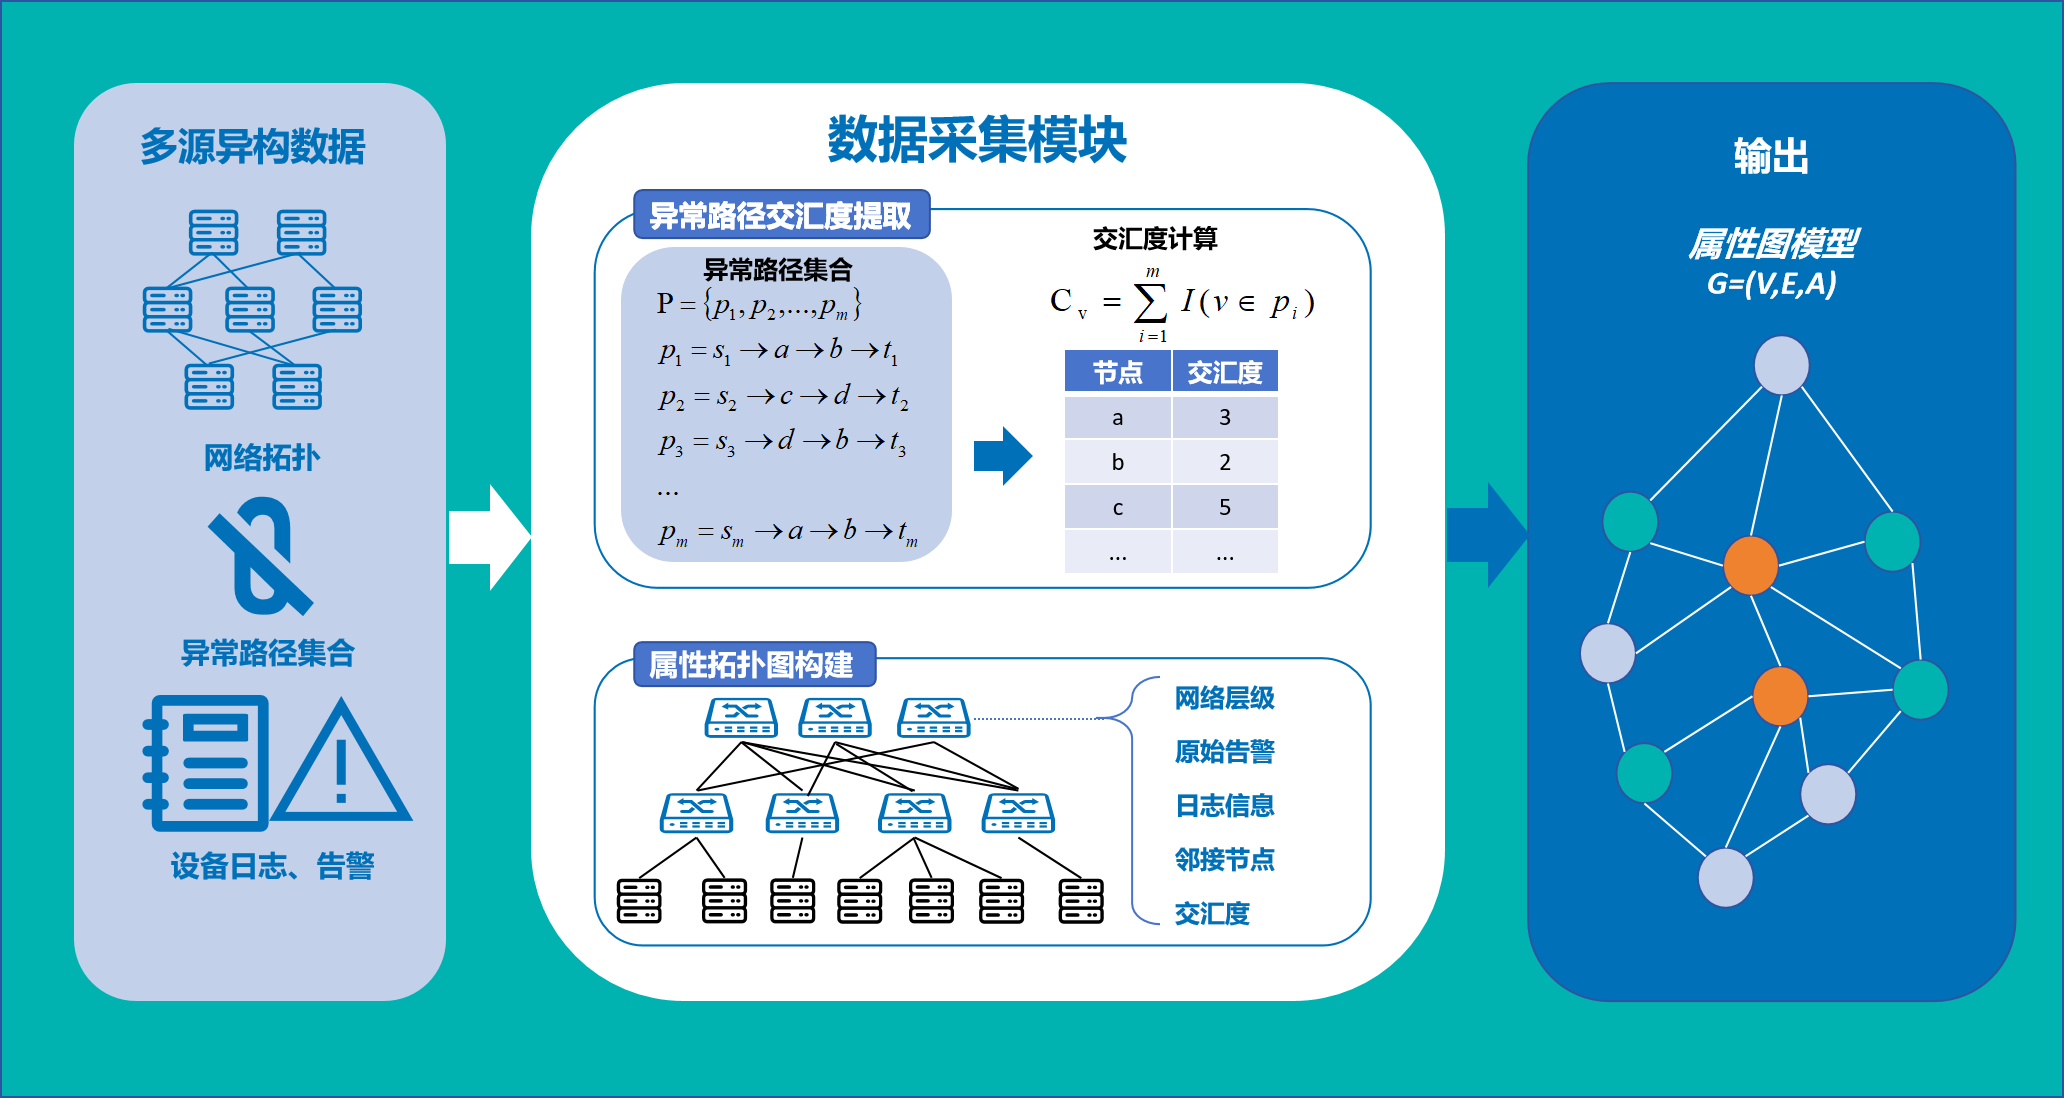
\includegraphics[width=120mm]{figures/mod1.png}
\caption{数据采集模块}
\label{fig:mod1}  % 给图像一个标签用于引用
\end{figure}

\subsection{异常路径探查与交汇度提取}
当Pingmesh系统触发告警时，设其返回的异常端到端探测路径集合为$P=\{p_1,p_2,\ldots,p_m\}$。由于数据中心网络普遍采用多路径等价路由，单点物理设备的故障往往会导致途经该设备的多条探测路径同时发生丢包。因此，本文定义节点的异常路径交汇度（Cross Count, $C_v$），即途经物理节点$v$的异常探测路径的总数：
\begin{equation}
C_v = \sum_{i=1}^{m} I(v \in p_i)
\end{equation}
其中，$I(\cdot)$为指示函数，当节点$v$属于异常路径$p_i$时为1，否则为0。
需要特别指出的是，节点的交汇度$C_v$值越大，并不等同于其为真实故障根因的嫌疑度越高。这一指标极易受到设备在网络拓扑中物理位置的影响。例如，核心层交换机（Spine）由于处于网络架构的枢纽位置，本身就承载了远超叶子节点（Leaf）的路由路径。当某个底层Leaf节点发生故障时，大量途径Spine并发往该Leaf的探查路径均会失败，从而导致原本健康的Spine节点被动呈现出极高的$C_v$值。

\subsection{属性拓扑图建模}

我们将指定时间窗口内的数据中心物理拓扑与告警数据联合建模为一个无向属性图 $G = (V, E, A)$。$V = \{v_1, v_2, \ldots, v_n\}$ 表示网络中所有物理设备（如Spine、Leaf、ToR交换机）的节点集合。$E \subseteq V \times V$ 表示设备之间的物理连接链路。$A$ 为节点属性集合。对于任意节点 $v \in V$，其属性 $A(v)$ 包含：节点的网络层级（Role）、承载的原始告警（Alarms）与日志（Logs）、邻接结点，以及计算得到的交汇度 $C_v$。通过上述建模，非结构化的多级网络事件被严密地绑定在了三维物理拓扑图谱中。

\section{拓扑剪枝模块}\label{sec:topo}
本模块是应对告警风暴并替大模型获取拓扑信息的核心组件。在告警风暴发生时，单点故障往往会引发海量的衍生告警。虽然引入运维专家的历史经验，为某些关键告警（如BGP邻居中断、端口Down）赋予高权重可以解决部分简单场景下的根因定位问题，但仅靠静态权重匹配的方法面临着严重的逻辑缺陷：由次生故障引发的告警同样可能具备极高的专家权重（例如，核心交换机Spine故障会导致下方数十台健康的叶子交换机Leaf报出高权重的路由中断告警）。本节详细阐述如何通过构建个性化向量并利用随机游走算法，实现嫌疑节点的初步筛选。

\subsection{专家知识引导的初始得分计算}\label{sec:ini}
为了表征不同节点在故障初期的嫌疑度，本文构建了一个多维度的评分函数，将其作为图计算的初始偏好向量。该过程分为权重映射与乘数放大两个阶段：

\subsubsection{1、基于告警优先级的初始得分}

系统首先加载预定义的告警优先级字典，提取节点 $v$ 承载的所有告警中优先级最高的一项 $W_{\max}$。若节点命中了高优告警，其初始得分 $E_v$ 由该优先级决定；若未命中权重表但存在告警，则根据告警数量 $N_{\text{alarm}}$ 赋予基准分。其逻辑定义如下：

\begin{equation}
E_v = 
\begin{cases}
W_{\max} & \text{if } W_{\max} > 0 \\[4pt]
2.0 \cdot N_{\text{alarm}} & \text{if } W_{\max} = 0,\ \text{存在告警} \\[4pt]
0.5 & \text{if 只存在日志，不存在告警}
\end{cases}
\end{equation}

\subsubsection{2、基于交汇度的乘数放大机制}

为识别处于多条失效路径交汇处的故障源，本文引入了乘数放大机制。只有当设备本身存在异常信号（$E_v > 0$）且其被异常路径经过（Cross Count $C_v > 0$）时，才显著放大其得分，防止健康的枢纽节点被误判。节点$v$的最终初始得分 $P_v$ 计算公式为：
\begin{equation}
P_v = 0.1 + E_v \cdot (1 + 0.5 \cdot C_v) + \delta_{\text{victim}}
\end{equation}
其中，$0.1$为平滑底分，$\delta_{\text{victim}}$为受害者补偿项（若节点为Pingmesh的源或目的IP，则赋予$0.5$的微弱增量，表征其受损状态）。

\subsection{个性化PageRank算法}
在确定了全网节点的初始得分向量 $\mathbf{p}$ 后，本文利用无向图 $G=(V,E)$ 表示设备间的物理连通性，并通过随机游走模型实现嫌疑权重在拓扑结构上的逻辑演进，本文采用个性化PageRank算法，其稳态概率分布 $\mathbf{r}$ 反映了在综合考虑拓扑关系与节点告警严重程度后的嫌疑度排名。迭代方程如下：
\begin{equation}
\mathbf{r}^{(t+1)} = (1 - \alpha) \mathbf{p}' + \alpha \mathbf{M} \mathbf{r}^{(t)}
\end{equation}
其中：$\alpha$ 为阻尼系数，本文取值 $0.85$，代表在图上游走的逻辑深度。$\mathbf{p}'$ 为\ref{sec:ini}节得到的得分向量 $\mathbf{p}$ 的归一化表示。$\mathbf{M}$ 为拓扑图的转移矩阵，描述了异常能量沿物理链路传播的可能性。通过该算法，原本分布在下游节点的次生告警权重，会沿着物理拓扑路径向拥有更高初始得分和更高交汇度的上游根因节点汇聚。

系统通过矩阵迭代直至达到稳态收敛（$\|\mathbf{r}^{(t+1)} - \mathbf{r}^{(t)}\| < \epsilon$）。最终，系统根据各节点的稳态得分进行降序排列，输出Top-10嫌疑节点列表。

截断值取10而非更小或更大的值，出于以下考虑：在告警风暴中，PageRank的稳态排序后得分最高的节点未必是真实根因，也可能是受影响最严重的下游设备。保留10个候选节点为后续大模型推理提供了充分的修正空间；同时，10个节点的规模是出于大模型上下文窗口容量的考虑，确保每个候选节点的关联告警与日志等语义信息均可被完整纳入提示词，不会因输入压缩而损失关键证据。使用上下文容量更充裕的大模型时，可以适当增加截断值。


\section{语义推理模块}

经过拓扑剪枝模块的PageRank计算，定位任务的搜索空间已从全局拓扑收敛至Top-10嫌疑节点。然而，PageRank的排序结果不能直接作为最终诊断，只是将范围缩小至Top-10之后，仍需在这组候选节点中确定哪一个才是根因。这一判断无法由PageRank自身完成，原因在于其两个固有局限。

第一，PageRank无法区分告警之间的因果方向。随机游走过程仅依赖物理连通性传播权重：当Spine故障导致下联Leaf上报BGP邻居中断时，Spine和Leaf的得分沿拓扑边相互传导、彼此增强。算法能识别这些节点存在关联，但因得分分布对称，无法判断是Spine导致Leaf告警，还是Leaf批量故障汇总到了Spine。

第二，PageRank将告警视为数值标签，无法理解告警语义。在专家权重初始化阶段，不同类型告警被赋予不同的分值，但这一映射是粗粒度的。例如，“RM\_DELETE\_DEFAULTRT”（默认路由删除）和“hwBfdSessUp”（BFD会话恢复）在权重表中可能被赋予相近数值，但在语义层面，前者是破坏性的操作型告警，后者仅是状态恢复通知，二者指向根因的力度截然不同。更一般地，运维中积累的领域经验（如“BFD会话频繁翻转暗示底层链路不稳定”）往往以自然语言形式沉淀在历史工单中，无法被编码进图算法的权重矩阵。

上述两个局限指向同一个结论：PageRank擅长回答“哪些节点在拓扑层面最可疑”，但不擅长回答“其中最可能为根因的是哪一个”。后一个问题需要理解告警的语义内容和网络协议的行为逻辑，这正是大语言模型的能力所在。

\subsection{大模型在最终定位中的作用}

在Top-10候选集上，LLM对每个候选节点的告警日志进行语义分析，结合对网络协议栈的理解，判断节点间的因果方向。例如，当Spine节点携带“端口Down”告警而Leaf节点携带“BGP邻居中断”告警时，LLM可依据协议层级推断前者是后者的原因；类似地，LLM能根据告警语义区分操作型告警与状态通知，删除路由比会话恢复的日志更可能指向故障源头。

最终，LLM输出一个列表，按照嫌疑从高到低排序，包含根因设备的IP地址及一段自然语言的诊断说明，描述其推理依据。这种可读的输出对运维人员具有直接参考价值。相比一个孤立的嫌疑节点排名，附带推理过程的诊断结论更有助于后续的止损和复盘。

\subsection{提示词设计}

LLM的推理质量依赖输入信息的组织方式。本文提示词设计遵循三个原则：

\textbf{搜索空间约束。}明确告知LLM，输入节点已经过拓扑剪枝模块的确定性筛选，根因在给定的Top-10节点之内，禁止超出候选集范围猜测。

\textbf{推理路径约束。}要求LLM先逐一分析每个候选节点的告警语义和设备层级，再进行节点间的因果比较，最后输出诊断结论，而非跳过分析直接给出猜测结果。

\textbf{输出格式约束。}要求以结构化JSON格式输出确诊设备IP和诊断说明，便于下游系统解析和呈现。

本文使用的核心提示词模板如下所示：


\begin{tcolorbox}[breakable,
    colback=gray!3, colframe=gray!60,
    title={\textbf{语义推理模块 提示词模板}},
    fonttitle=\bfseries, fontupper=\small,
    arc=1mm, left=6pt, right=6pt, top=6pt, bottom=6pt]
\begin{lstlisting}[basicstyle=\small\ttfamily, breaklines=true, xleftmargin=0pt, resetmargins=true, language={}, escapeinside={(*@}{@*)}]
##(*@\textbf{角色设定}@*)
你是一名数据中心网络排障专家，熟悉Pingmesh拨测原理、
网络拓扑结构及常见网络协议的故障行为。
##(*@\textbf{任务目标}@*)
根据以下Top-10嫌疑节点数据（NODES）
和Pingmesh告警信息（INFO），确定最可能的根因设备。
注意：根因必然在给定的Top-10节点内，不得向外猜测。
##(*@\textbf{推理准则}@*)
逐一分析每个候选节点的告警类型和语义，
判断其是根因型告警还是衍生型告警。
结合设备在网络拓扑中的角色（Spine/Leaf），
推断告警之间的因果方向，输出最可能的根因设备。
##(*@\textbf{输出格式}@*)
严格以JSON格式输出：
  "diagnoses": [{
    "ip": "确诊设备IP",
    "explanation": "诊断依据"
    }]
(*@\textbf{## 输入数据}@*)
1. INFO（Pingmesh告警信息）：{INFO}
2. NODES（Top-10节点拓扑与状态数据）：{NODES}
\end{lstlisting}
\end{tcolorbox}

\chapter{实验及分析}
本章旨在通过充分的实验验证本文所提出的“基于Pingmesh触发、PageRank拓扑剪枝与LLM深度推理相协同的大规模网络根因定位方案”的故障定位与故障诊断能力。我们将详细介绍实验所使用的数据集、评价指标以及基线方法，并分别在常规场景和告警风暴场景下进行深入的对比分析与消融实验。
\section{数据集与实验配置}
\subsection{数据集介绍}

实验数据集来源于华为云生产环境的历史故障案例，时间跨度为2025年9月至2025年12月，共计104例。
数据集依据单次故障触发的全网总告警数划分为常规场景与告警风暴场景两类。以告警总数作为划分标准，直接对应告警风暴的定义性特征：告警风暴区别于普通故障的本质在于告警数量的爆发式增长，而非故障类型的差异。采用告警总数作为划分依据，能够客观、可复现地衡量根因定位任务的难度。

600条告警的阈值根据本文所用大语言模型DeepSeek-R1-Distill-Qwen-32B的上下文窗口容量确定。该模型基于Qwen2.5-32B架构，最大上下文长度为131,072 tokens。在本系统的提示词格式下，每条告警信息约消耗200个token，包含设备IP、告警类型、严重级别、告警描述文本以及该设备邻接节点信息。按此估算，600条告警总计约消耗12万tokens，已逼近上下文窗口上限。当单次故障触发的告警数超过600条时，将全部告警直接送入LLM进行端到端推理在工程上不再可行：模型无法在单一上下文中容纳全部告警，而分段处理又会因上下文截断破坏告警间的因果关联。

按此标准划分后，常规场景共90例，告警风暴场景共14例，二者对比如表\ref{tab:scenario_compare}所示。

\begin{table}[H]
\centering
\caption{常规场景与告警风暴场景对比}
\label{tab:scenario_compare}
\begin{tabular}{p{2.2cm}p{5.2cm}p{5.2cm}}
\toprule
 & \textbf{常规场景} & \textbf{告警风暴场景} \\
\midrule
样本数量 & 90例 & 14例\\
\hline
告警数量 & $\leq 600$条 & $> 600$条\\
\hline
故障范围 & 孤立故障或局部异常 & 核心设备故障引发级联传播\\
\hline
告警特征 & 衍生告警较少，易于定位 & 多层级告警同时爆发\\
\bottomrule
\end{tabular}
\end{table}


\subsection{实验环境及配置}

本研究的所有实验均基于一台华为昇腾（Ascend）AI服务器构建，其详细硬件配置与软件环境如表~\ref{tab:experimental-setup}所示。软件栈核心基于PyTorch与昇腾NPU架构，并采用vLLM框架及其昇腾插件作为大模型（LLM）的推理引擎。

\begin{table}[htbp]
    \centering
    \caption{实验环境配置}
    \label{tab:experimental-setup}
    \small
    \begin{tabularx}{\textwidth}{llX}
        \toprule
        \textbf{类别} & \textbf{项目} & \textbf{规格/信息} \\
        \midrule
        \textbf{硬件} & CPU & 华为鲲鹏920 (Kunpeng-920)，4路，共256核\\
        & 内存 & 2 TB \\
        & NPU & 8 $\times$ 华为昇腾910B3 (单卡64 GB HBM) \\
        \midrule
        \textbf{操作系统} & 发行版 & Ubuntu 22.04 LTS \\
        & 内核 & 5.15.0-119-generic \\
        \midrule
        \textbf{关键软件} & Python & 3.10.16 \\
        & PyTorch & 2.5.1 (搭配torch-npu 2.5.1) \\
        & vLLM & 0.7.3 (含vllm\_ascend 0.7.3.post1插件) \\
        & Transformers & 4.57.1 \\
        & 其他依赖 & LangChain 0.3.12, NumPy 1.26.4, pandas 2.3.3 \\
        \midrule
        \textbf{推理模型} & 模型架构 & DeepSeek-R1-Distill-Qwen-32B（Dense，总参数32B）\\
        & 部署方式 & 基于vLLM Ascend插件进行分布式并行推理\\
        \bottomrule
    \end{tabularx}
\end{table}

\noindent \textbf{补充说明}：服务器搭载8枚华为昇腾910B3 NPU，推理配置参数遵循官方建议：Temperature设为0.6，最大生成长度为32,768 tokens，且不使用系统提示词。
\subsection{评价指标}

对于根因定位任务，本文采用智能运维领域广泛使用的\textbf{Top-$k$ 准确率}（Top-$k$ Accuracy）作为核心评价指标。系统对每个故障实例输出一个按嫌疑度降序排列的候选节点列表 $P_{i,[1:K]}$，其中 $K$ 为列表长度。设 $g_i$ 为第 $i$ 个故障实例的真实根因节点，$N$ 为故障实例总数，则Top-$k$ 准确率定义为：

\begin{equation}
\text{Top}k = \frac{1}{N} \sum_{i=1}^{N} \mathbb{I}\bigl(g_i \in P_{i,[1:k]}\bigr)
\end{equation}

其中 $\mathbb{I}(\cdot)$ 为指示函数，$k$ 一般取1、2、3，分别表示：真实根因恰好排在嫌疑列表第1位的命中率（Top-1 Acc），以及根因落入前3位的覆盖率（ Top-3 Acc）。在大规模排障中，将排查范围缩小至前3个节点即可极大节省人工排查时间，具有较高的工程落地价值。
\section{基线方法与对比实验}
\subsection{基线方法选择}

为验证本文提出方法的先进性，我们选取了学术界与工业界在网络与微服务系统根因定位领域的三种代表性前沿工作作为基线（Baseline）进行对比：


 \textbf{TraceRCA\upcite{li_practical_2021}}：该方法的核心思想源自频谱故障定位，即“根因微服务所在的调用链路，会表现出更多的异常Trace和更少的正常Trace”。其技术路径分为三步：首先，通过多指标调用异常检测筛选出异常Trace；其次，利用频繁模式挖掘算法（如FP-Growth）找出异常Trace高频经过的微服务候选集；最后，结合Jaccard相似系数和异常传播方向动态推断，对候选微服务进行打分排序。该方法本质上是一种统计方法，通过统计异常Trace在各微服务上的分布来推断根因，原始论文面向微服务系统，但其统计建模思路在DCN场景下同样成立，只需将异常微服务调用链集合映射为异常端到端路径集合，从而进行dcn场景中的根因定位。该方法完全不依赖告警日志数据。

\textbf{NetEventCause\upcite{yuan_neteventcause_2025}}：该方法将告警事件流建模为多变量时序点过程，利用神经常微分方程（ODE-RNN）学习历史告警对当前时刻各类型告警强度的复杂激励关系，突破了传统霍克斯过程强假设的限制。在推理阶段，它通过贝叶斯推断对比“先验根因强度”与“历史事件触发的条件强度”来区分根因与衍生告警，并引入可解释性AI中的积分梯度归因方法来量化告警之间的格兰杰因果关系，从而还原异常传播链。

 \textbf{BiAn\upcite{wang_towards_2025}}：业界最新的纯大语言模型检索引擎框架，代表了将LLM应用于网络运维的工业级尝试。该框架不直接端到端处理原始日志，而是设计了一套模拟运维专家排障思维链的分层多智能体架构：首先利用微调小模型对海量监控告警进行分类摘要；其次，按照标准作业程序对单设备进行异常分析；最后结合网络拓扑和事件时间线进行多流水线综合打分，定位故障设备。为了适应网络演进，BiAn还设计了基于LLM反思与知识固化的持续提示词更新机制，以解决大模型在复杂运维数据上的幻觉与推理随机性问题。


各种方法在常规场景和告警风暴场景数据集上的对比实验结果如表~\ref{tab:comparison}所示。

\begin{table}[htbp]
\centering
\caption{本文方法与各基线方法的定位准确率对比}
\label{tab:comparison}
% 使用resizebox自动适应页面宽度
\resizebox{\textwidth}{!}{%
\begin{tabular}{@{}ll @{\qquad} cc @{\qquad} cc @{\qquad} c@{}}
\toprule
& & \multicolumn{2}{c}{常规场景} & \multicolumn{2}{c}{告警风暴场景} & \\
\cmidrule(lr){3-4} \cmidrule(lr){5-6}
\textbf{方法} & \textbf{方法类型} & \textbf{Top-1 (\%)} & \textbf{Top-3 (\%)} & \textbf{Top-1 (\%)} & \textbf{Top-3 (\%)} & \textbf{耗时(s)} \\
\midrule
TraceRCA & Trace路径统计学 & 14.44 & 24.44 & 7.14 & 7.14 & 0.0013 \\
NetEventCause & 无拓扑时序点过程 & 60.00 & 86.67 & 14.29 & 28.57 & 0.0010 \\
BiAn & 纯LLM检索引擎 & 48.89 & 67.78 & 21.43 & 35.71 & 21.3030 \\
本文方法 & 综合推理 & \textbf{60.00} & \textbf{92.22} & \textbf{35.71} & \textbf{78.57} & 9.9954 \\
\bottomrule
\end{tabular}%
}
\end{table}
\subsection{实验结果分析}

在常规场景中，本文方法在Top-1和Top-3准确率上均取得最优结果。与最优基线方法NetEventCause相比，Top-3提升了6.4\%；Top-1则与NetEventCause持平，这是因为在告警数量较少、拓扑结构清晰的常规场景下，时序点过程模型已能从告警序列中较准确地捕捉因果信号，本文方法在命中精度上的额外优势有限。基于拓扑网络结构进行分析的TraceRCA由于完全缺乏告警语义信息，仅依赖路径异常比例进行统计推断，两项指标均垫底。BiAn虽然具备语义理解能力，但缺乏对网络拓扑结构的精确感知，其多Agent间的信息流转以自然语言文本为载体，无法对设备间的空间关系进行精确计算，Top-1仅为48.89\%。

在告警风暴场景中，所有方法的性能均明显下降，但本文方法的降幅远小于各基线方法。NetEventCause的Top-1准确率从60.00\%骤降至14.29\%，降幅高达76.2\%，BiAn的Top-1准确率从48.89\%降至21.43\%，降幅达56.2\%，而本文方法仅从60.00\%降至35.71\%，降幅为40.5\%。与告警风暴场景中表现最好的基线BiAn相比，本文方法的Top-1和Top-3准确率分别高出66.6\%和120.0\%。这一显著差异源于本文方法的降维机制：PageRank拓扑剪枝模块在LLM推理之前已将告警风暴中的数千条告警压缩为Top-10候选节点列表，使LLM的推理对象从海量告警缩减为10个嫌疑设备，从而在上下文窗口容量以内完成语义推理。NetEventCause的纯时序建模在海量并发衍生告警中无法区分因果方向，告警风暴中数十种类型的告警几乎同时爆发，时序点过程模型学习到的条件强度函数在此时退化为均匀分布，根因信号完全淹没。BiAn虽然引入了语义理解，但其三阶段Agent架构缺乏拓扑网络理解环节：所有告警经信息提取Agent转化为结构化摘要后仍全部进入后续推理流程，当告警数量超出上下文窗口容量时，模型注意力在大量非根因告警中分散，推理准确率随之急剧下降。本文方法在告警风暴场景中的Top-3达到78.57\%，这意味着在超过四分之三的告警风暴案例中，根因设备位于系统输出的前3个候选节点之内，具备实用化的工程落地潜力。

从时间效率角度看，四类方法呈现出明显的两极分化。TraceRCA和NetEventCause的单案例推理时间分别为0.0013秒和0.0010秒，属于毫秒级轻量方法，其计算开销几乎可以忽略，这是纯统计方法在工程部署中的固有优势。两类LLM方法的推理时间则进入了秒级：BiAn为21.30秒，本文方法为9.99秒，本文方法的推理速度是BiAn的2.13倍。BiAn耗时较高的原因在于其三阶段多智能体架构——告警分类摘要、单设备异常分析、多流水线综合打分三个环节各自需要一次LLM推理调用，累计推理量远超单次调用。本文方法的PageRank拓扑剪枝将LLM的推理输入从全量告警压缩为Top-10候选节点的结构化摘要，仅需一次LLM推理即可完成根因定位，因而推理时间不到BiAn的一半。综合精度与时间两个维度，本文方法在LLM类方法中实现了更优的平衡。

\section{消融实验}
\subsection{实验设计}
为了深入解析本文方案中各个核心模块（专家告警权重、PageRank拓扑剪枝、LLM语义推理）对整体根因定位性能的具体贡献，我们设计了四组消融模型进行充分验证：
\begin{itemize}
    \item \textbf{LLM}：去除拓扑剪枝和告警权重，将收集到的关联原始告警直接输入给大语言模型进行推理。
    \item \textbf{LLM + 告警权重}：引入专家知识的告警优先级权重，对告警进行一定程度的启发式过滤后，再交由大语言模型推理。
    \item \textbf{PageRank}：纯数学图算法范式。仅使用本文\ref{sec:topo}介绍的基于告警特征初始化的个性化PageRank算法进行拓扑游走降维，直接输出稳态收敛得分排名，完全不使用LLM。
    \item \textbf{LLM + 告警权重 + PageRank}：本文完整的端到端根因定位方案。
\end{itemize}

消融实验的各项准确率指标对比详情如~\ref{tab:ablation}所示。

\begin{table}[htbp]
\centering
\caption{本文方法各组件的定位准确率对比}
\label{tab:ablation}
\resizebox{\textwidth}{!}{%
\begin{tabular}{@{}l @{\qquad} cc @{\qquad} cc @{\qquad} c@{}}
\toprule
& \multicolumn{2}{c}{常规场景} & \multicolumn{2}{c}{告警风暴场景} & \\
\cmidrule(lr){2-3} \cmidrule(lr){4-5}
\textbf{方法组合} & \textbf{Top-1 (\%)} & \textbf{Top-3 (\%)} & \textbf{Top-1 (\%)} & \textbf{Top-3 (\%)} & \textbf{耗时(s)} \\
\midrule
LLM                               & 51.11 & 75.56 & 7.14  & 21.43 & 9.9035\\
LLM+告警权重                       & 54.40 & 85.56 & 28.57 & 42.86 & 9.9906\\
PageRank                           & 38.89 & 77.78 & 28.57 & 64.29 & 0.0264 \\
LLM+告警权重+PageRank              & 60.00 & 92.22 & 35.71 & 78.57 & 9.9954 \\
\bottomrule
\end{tabular}%
}
\end{table}

\subsection{消融实验分析}

LLM单独使用时，在常规场景中Top-1准确率为51.11\%，但在告警风暴场景中骤降至7.14\%，降幅高达86.0\%。这一断崖式下跌与第三章需求分析的判断一致：当告警数量远超上下文窗口容量时，模型注意力在数千条告警文本中高度分散，无法对设备间的拓扑关系进行有效追踪，推理几乎失效。

引入专家告警权重后，告警风暴场景的Top-1准确率从7.14\%提升至28.57\%，这验证了专家先验知识有助于区分根因告警与衍生告警。但LLM+告警权重在告警风暴场景中Top-1准确率仅为28.57\%，说明静态权重规则能够抬高根因型告警的初始分值，但当前根因与次生故障触发同类高优告警时（如大面积BGP邻居中断同时出现在根因设备和健康下游设备上），权重机制无法区分孰为因、孰为果。

PageRank单独使用时展现出与LLM互补的性能特征。在常规场景中Top-1准确率仅38.89\%，比朴素LLM低12.22个百分点，缺乏语义区分能力使其无法精确命中根因。但在告警风暴场景中，PageRank的Top-1准确率达到28.57\%（与LLM+告警权重持平），Top-3准确率达到64.29\%（超出LLM+告警权重50\%）。这一反差说明：图上随机游走不依赖上下文窗口大小，其推理质量不受告警数量增长的影响；在告警风暴中，图算法能够利用物理拓扑连通性将异常权重汇聚至被多条异常路径共同穿越的节点，而这一计算是LLM单靠文本推理无法完成的。

本文完整方案（LLM+告警权重+PageRank）在所有指标上均取得最优结果。与未使用PageRank的LLM+告警权重相比，告警风暴场景中Top-1准确率从28.57\%提升至35.71\%，Top-3准确率从42.86\%提升至78.57\%；与未使用LLM的PageRank相比，常规场景中Top-1从38.89\%提升至60.00\%。这两个方向上的显著提升揭示了两模块之间的分工互补关系。PageRank负责拓扑空间的降维，从数百个节点中提取Top-10候选集，使LLM的推理输入始终控制在上下文窗口容量以内；LLM负责语义空间的根因定位，在压缩后的10个候选节点上，利用其对告警文本和网络协议行为的理解，判断节点间的因果方向。两者各自承担擅长的工作，各自不擅长的问题由对方补齐。

从时间开销来看，四个变体的单案例推理时间揭示了各模块的计算代价。PageRank单独使用时仅耗时0.0264秒，不到任何含LLM变体的0.3\%。包含LLM的三个变体（LLM、LLM+告警权重、LLM+告警权重+PageRank）的推理时间均在9.90至10.00秒之间，差异不超过0.1秒。这一数据说明两个事实。第一，整个系统的时间瓶颈在LLM推理，PageRank和专家权重的计算开销可以忽略不计。第二，PageRank剪枝并未增加系统的时间负担——它在告警风暴场景中将Top-1准确率从7.14\%提升至35.71\%（提升400\%），而额外引入的时间成本仅为0.09秒，不到总耗时的1\%。PageRank以近乎零的时间代价换取了告警风暴场景中四倍的精度提升，证明拓扑剪枝是一种高性价比的降维策略。

\section{不同基座模型的性能对比}

前述实验均以DeepSeek-R1-Distill-Qwen-32B作为大语言模型基座。为了评估本文方案对不同基座模型的鲁棒性，以及模型规模与推理能力对根因定位精度的影响，本节在相同的实验设置下，采用五种模型进行对比：DeepSeek-R1-Distill-Qwen-7B、DeepSeek-R1-Distill-Qwen-14B、DeepSeek-R1-Distill-Qwen-32B、Qwen2.5-14B-Instruct和Qwen2.5-32B-Instruct。其中前三者属于DeepSeek-R1蒸馏系列，后二者为Qwen2.5原生指令微调系列。通过跨系列、跨规模的对比，可以分别观察推理能力与参数规模对最终根因定位精度的影响。

实验配置与前文保持一致：PageRank剪枝环节的拓扑剪枝策略和专家权重表不做任何调整，仅替换基座大模型，提示词模板不变。实验结果如表\ref{tab:backbone}所示。


\begin{table}[htbp]
    \centering
    \caption{不同基座模型下的根因定位准确率对比}
    \label{tab:backbone}
    \resizebox{\textwidth}{!}{%
    \begin{tabular}{@{}ll @{\qquad} cc @{\qquad} cc @{\qquad} c@{}}
    \toprule
    & & \multicolumn{2}{c}{常规场景} & \multicolumn{2}{c}{告警风暴场景} & \\
    \cmidrule(lr){3-4} \cmidrule(lr){5-6}
    \textbf{基座模型} & \textbf{参数量} & \textbf{Top-1 (\%)} & \textbf{Top-3 (\%)} & \textbf{Top-1 (\%)} & \textbf{Top-3 (\%)} & \textbf{耗时(s)} \\
    \midrule
    DeepSeek-R1-Distill-Qwen-7B  & 7B  & 12.22 & 21.11 & 0.00  & 0.00  & 11.5539 \\
    DeepSeek-R1-Distill-Qwen-14B & 14B & 47.78 & 71.11 & 7.14  & 14.29 & 15.3409 \\
    DeepSeek-R1-Distill-Qwen-32B & 32B & 60.00 & 92.22 & 35.71 & 78.57 & 9.9954 \\
    Qwen2.5-14B-Instruct        & 14B & 42.22 & 56.67 & 7.14  & 14.29 & 11.3458 \\
    Qwen2.5-32B-Instruct        & 32B & 53.33 & 75.56 & 14.29 & 21.43 & 13.2144 \\
    \bottomrule
    \end{tabular}%
    }
    \end{table}
\subsection{实验结果分析}

\textbf{1. 模型规模对定位精度的影响。}

从DeepSeek-R1蒸馏系列的纵向对比中可以清晰地观察到参数规模对根因定位精度的影响。在常规场景中，7B模型的Top-1准确率仅为12.22\%，14B跃升至47.78\%，相对提升291\%，32B进一步提升至60.00\%，相对14B提升25.6\%。这一增长轨迹说明：从7B到14B的提升是质变性的，7B模型基本不具备可靠的根因定位能力，14B模型已能达到中等可用水平；从14B到32B的提升则是精细化的，在已有较高基线之上的进一步优化。Qwen2.5-Instruct系列呈现类似趋势：14B的Top-1准确率为42.22\%，32B为53.33\%，提升幅度为26.3\%。

在告警风暴场景中，规模的影响更加明显。DeepSeek-R1系列中，7B模型在告警风暴场景的两项指标全部为零，面对超过600条告警的输入时，7B模型完全无法区分因果方向，即便放宽至Top-3准确率也无法覆盖真实根因。14B模型的告警风暴场景Top-1准确率为7.14\%，32B模型则达到35.71\%。从14B到32B在告警风暴场景中提升400\%，远大于常规场景中的25.6\%，这表明大模型对告警风暴的承受能力存在一个规模门槛，低于该门槛时性能断崖式下跌，越过门槛后才能维持基本的推理能力。

\textbf{2. R1蒸馏推理能力的贡献。}

对比同规模的DeepSeek-R1-Distill与Qwen2.5-Instruct，可以剥离推理链蒸馏对根因定位的净增益。在14B级别，R1蒸馏的常规场景Top-1准确率为47.78\%，比Qwen2.5-Instruct的42.22\% 高出5.56个百分点，相对提升13.2\%；Top-3准确率为71.11\% 对56.67\%，差距扩大至14.44个百分点。在告警风暴场景中，两者的Top-1和Top-3准确率持平，分别为7.14\%和14.29\%，表明14B级别下R1蒸馏的推理链能力尚不足以在极端场景中提供实质增益。

在32B级别，R1蒸馏的优势进一步放大且呈现场景分化特征。常规场景中，R1-32B的Top-1准确率比Qwen2.5-32B高出6.67个百分点，相对提升12.5\%，差距与14B级别相近。但在告警风暴场景中，R1-32B的Top-1准确率35.71\% 是Qwen2.5-32B的14.29\% 的2.5倍，Top-3准确率78.57\% 是后者21.43\% 的3.7倍。两组数据的对比揭示了一个规律：R1蒸馏的推理链能力在常规场景下提供的增益相对稳定，约在12\% 至13\% 之间，但在告警风暴场景下，其价值随参数规模的增大而急剧放大。14B级别下R1蒸馏未能挽救告警风暴性能，二者的Top-1准确率相同，32B级别下则形成了质的差距。这说明在复杂的告警风暴场景下，推理链蒸馏的优势更能体现，并且随着模型规模的增大，推理链蒸馏带来的增益越发明显。

\textbf{3. 告警风暴场景下的模型退化特征。}

所有模型在告警风暴场景中均出现显著的性能退化，但退化幅度差异悬殊。按常规场景到告警风暴场景的Top-1准确率降幅排序：DeepSeek-R1-7B退化100\%，从12.22\% 直接归零；Qwen2.5-14B退化83.1\%；DeepSeek-R1-14B退化85.1\%；Qwen2.5-32B退化73.2\%；DeepSeek-R1-32B退化40.5\%。退化幅度与参数规模和推理能力均呈负相关。规模越大、具备推理链蒸馏的模型，在告警风暴中维持推理质量的能力越强。

7B模型的完全失效值得单独讨论。该模型在告警风暴场景中Top-1和Top-3准确率均为0.00\%，这意味着在14个告警风暴样本中，它从未将真实根因排入前3名。这与第三章讨论的上下文过载机制一致：7B模型的上下文窗口与更大规模模型相同，均为131K tokens，但其注意力机制在长上下文中对关键信息的捕捉能力远弱于后者。当600条告警同时输入时，7B模型的注意力分布趋于均匀化，无法聚焦于携带破坏性语义的关键告警，最终输出近乎随机猜测的结果。

\textbf{4. 综合推荐与工程权衡。}

从精度角度看，DeepSeek-R1-Distill-Qwen-32B在所有指标上全面领先，尤其是在告警风暴场景中的优势不可替代。如果部署场景对最差情况下的定位能力有严格要求，32B规模的R1蒸馏模型是唯一能够同时满足常规和告警风暴双场景精度要求的选项。如果存在GPU显存或推理延迟的硬约束，常规场景占数据集主体的90/104，在该场景下DeepSeek-R1-14B的Top-3准确率为71.11\%，Qwen2.5-32B的Top-3为75.56\%，表现接近；但告警风暴场景中Qwen2.5-32B的Top-3准确率21.43\% 显著高于DeepSeek-R1-14B的14.29\%，资源受限时优先保证参数规模在告警风暴场景中更具实际价值。

从时间角度看，五种模型的单案例平均推理时间如表~\ref{tab:backbone}末列所示，总体差异不大。Qwen2.5-Instruct系列的时间随规模递增（14B 11.35秒、32B 13.21秒），符合直觉。DeepSeek-R1蒸馏系列则不同：14B耗时15.34秒，比同规模Instruct模型慢35.2\%；32B仅耗时9.99秒，反比Instruct模型快24.4\%。这是因为R1蒸馏模型的推理链长度随规模变化——14B推理能力偏弱，思考链冗长、反复推敲，token总数膨胀；32B推理能力足够强，思考链精准简洁，token总数被压缩，总时间反而最低。在32B级别，R1蒸馏不再需要在精度和速度之间权衡，两者同步占优。综合精度与时间，DeepSeek-R1-Distill-Qwen-32B在所有候选模型中Top-1准确率最高（常规场景60.00\% / 告警风暴场景35.71\%）、推理时间最短（9.99秒），是本方案的最优基座选择。

综合消融实验与基座模型对比的结果，可以归纳出两条对工程部署有指导意义的结论。第一，PageRank拓扑剪枝是本方案中性价比最高的组件：它以0.026秒的计算开销换取了告警风暴场景中Top-1准确率从7.14\% 到35.71\% 的提升，且这一增益在不同基座模型上稳定复现。第二，系统的性能下限由PageRank保障，上限由LLM决定：即使使用性能最弱的7B模型，系统在常规场景中的Top-3仍可达21.11\%，高于完全移除PageRank后的告警风暴表现；但要将告警风暴Top-3推至78.57\%，则需要32B级别且具备推理链蒸馏的模型。这一分工意味着该方案可以通过升级LLM基座持续获得精度提升，而无需调整PageRank和专家权重机制。

\chapter{案例分析}

本节从数据集中选取了两个案例，分别展示本文方案中两类组件各自的必要性。第一个案例说明纯大语言模型在处理多跳拓扑关系时容易出错，引入PageRank剪枝的必要性；第二个案例说明纯图算法在多路径得分趋同时无法区分根因，引入大语言模型语义推理的必要性。

% ---------- 第一节 ----------
\section{案例一：拓扑盲区导致的大语言模型误判}

2025年10月28日14:32:10，Pingmesh系统在亚太区吉隆坡机房检测到Pod间网络异常：源IP \texttt{10.64.250.21}到目的IP \texttt{26.63.1.7}之间出现14.0\% 的持续丢包。该告警属于端到端探测层面的异常检测结果，并非故障的第一现场。回溯同一时间窗口内的设备告警序列，可以还原出一条清晰的因果链路：

\begin{itemize}
    \item \textbf{14:31:52} \quad Leaf交换机\texttt{11.64.255.250}（Leaf层，直接接入服务器）上报\texttt{RM\_DELETE\_DEFAULTRT}（默认路由删除）。该告警属于操作型（DELETE），具有明确的破坏性语义，且时间上最先出现。
    \item \textbf{14:31:55} \quad 同一Leaf交换机上报BGP邻居中断。路由表被删除后BGP对等体关系随之破裂，是根因操作在协议层的直接连锁反应，时间紧随根因操作且位于同一设备。
    \item \textbf{14:31:56} \quad 同一Leaf交换机上报\texttt{hwBfdSessUp}（BFD会话反复翻转）。转发平面受路由删除影响后，链路检测协议出现反复振荡，是转发层异常的直接信号。
    \item \textbf{14:32:02} \quad 邻接防火墙\texttt{11.64.255.253}（网络安全设备，拓扑上位于Leaf交换机的下游）上报IPv4默认路由变更。由上游Leaf的路由删除事件经由拓扑邻接关系触发，时间滞后10秒且设备角色为下游，属于次生事件。
    \item \textbf{14:32:10} \quad Pingmesh探测到源\texttt{10.64.250.21}→目的\texttt{26.63.1.7}丢包14.0\%。端到端探测对已发生故障的最终感知结果，时间最晚（滞后根因操作18秒），属于故障在应用层面的表现而非原因。
\end{itemize}

从告警时间线可以清晰得出三个判断。第一，所有告警的时间零点在Leaf交换机\texttt{11.64.255.250}，其上最先出现具有破坏性语义的操作型告警，后续告警均为其连锁反应，这是因果方向的基本依据。第二，从设备角色看，\texttt{11.64.255.250}是唯一的Leaf层接入设备，处于故障传播链的最上游——BGP中断和BFD翻转均发生在同一设备上，而防火墙和Pingmesh端点的告警分别位于拓扑下游和应用感知层，时间上的先后与拓扑上的上下游关系完全吻合。第三，从告警类型看，操作型告警（DELETE）和协议中断告警（BGP Down）指示根因的能力远强于状态变更通知型告警（路由变更、丢包率异常），前者是故障的主动触发动作，后者仅是被动感知结果。

真实根因是：交换机\texttt{11.64.255.250}误删了默认路由，导致途经该设备的四条端到端路径发生丢包，上层业务流在不知情的情况下被持续丢弃。

\subsection{直接使用大语言模型的结果}

将包含Pingmesh告警信息、设备告警的、Syslog日志原文、拓扑邻接关系的原始信息全部不加筛选地直接输入大语言模型，模型输出的诊断结论是：根因在源和目的节点本身。

\begin{quote}\itshape
    “源节点\texttt{10.64.250.21}和目标节点\texttt{26.63.1.7}没有日志或告警。发现有两台防火墙和交换机（\texttt{11.64.255.250}等）有BFD和路由变化告警，但缺乏直接证据使得难以确定它们是否是根本原因…… 因此综合考虑，最可能的问题节点就是源和目标节点本身，因为它们直接参与了Pingmesh测试…… 导致丢包。”
\end{quote}

这个结论是错误的。错误的原因不在于模型不理解告警的语义，它正确识别了\texttt{RM\_DELETE\_DEFAULTRT}是路由删除操作、\texttt{hwBfdSessUp}是BFD会话状态变化。问题在于，模型无法在拓扑空间中建立源IP经过交换机到达目的IP的物理路径关系，当面对多台设备的连接关系和告警信息时，大语言模型只能在文本层面进行关键词关联。而且，LLM在未经过拓扑剪枝压缩的全量输入中，无法从数百条混杂信息里有效提取这一模式。Pingmesh告警的文本中最显眼的字段是源IP和目的IP，模型据此将注意力集中在这两个端点上，忽略了真正承载流量的中间交换机。

\subsection{引入PageRank剪枝后的处理流程}

本文方案的处理流程分为两步：PageRank先对拓扑图进行剪枝，大语言模型再对压缩后的候选集进行语义复核。

在PageRank阶段，交换机\texttt{11.64.255.250}的拓扑位置决定了它的嫌疑度远高于其他节点：它被全部4条异常Pingmesh路径共同穿越，在随机游走过程中持续从多条异常端点接收权重；它同时命中了高权重告警\texttt{RM\_DELETE\_DEFAULTRT}（专家权重60分），个性化向量进一步放大了其稳态得分。迭代收敛后，\texttt{11.64.255.250}的综合嫌疑度为53.48分，位列全网第一。作为对比，源IP \texttt{10.64.250.21}和目的IP \texttt{26.63.1.7}的嫌疑度均在9分以下，它们仅各自被1条异常路径覆盖，且未匹配到任何高权重告警。

大语言模型复核阶段，模型接收到的输入不再是数百个节点的原始日志，而是经PageRank排序后的Top-10节点及其结构化摘要。此时模型注意到两个关键信息：第一，\texttt{11.64.255.250}的嫌疑度是第二名的三倍以上，差距悬殊；第二，该节点关联的\texttt{RM\_DELETE\_DEFAULTRT}是明确的破坏性操作告警，而非状态通知。模型最终输出的诊断结论为\texttt{11.64.255.250}是根因设备，并明确指出源和目的IP仅为Pingmesh探测端点，不构成故障原因。

\subsection{分析}

本案例展示了大语言模型在根因定位中的一个结构性缺陷：它不具备对网络拓扑的精确感知能力。模型能区分一条告警是路由删除还是状态恢复，却无法计算一个节点被几条异常路径穿越。当告警文本中显式出现的实体（如Pingmesh的源目的IP）与真正的故障节点不一致时，模型倾向于相信文本中直接可见的信息，而非从拓扑结构中推导出的隐含关系。

PageRank弥补了这一缺陷。基于图上随机游走的拓扑剪枝不依赖文本理解，而是通过确定性计算将异常权重汇聚到被多条路径共同穿越的节点上。剪枝后的输出将大语言模型的推理范围从数百个节点压缩为少量高分候选，并且用数值化的嫌疑度替代了模糊的文本关联，使模型不再被Pingmesh告警中的端点信息误导。

% ---------- 第二节 ----------
\section{案例二：PageRank得分趋同}

2025年10月29日09:15:30，华北乌兰察布机房出现Pingmesh丢包异常。回溯同一时间窗口内的设备告警序列，可以观察到一条以Core层交换机为起点的故障传播链：

\begin{itemize}
    \item \textbf{09:15:03} \quad Core交换机\texttt{11.67.128.64}（Core层，全网路由枢纽，连接数十台Leaf交换机）上报\texttt{hwLocalFaultAlarm\_active\_for\_CND}（本地硬件故障告警）。硬件层异常，属于物理故障信号，时间上最先出现，且告警文本描述明确指向本地硬件故障。
    \item \textbf{09:15:05} \quad 同一Core交换机上报\texttt{RM\_DELETE\_DEFAULTRT}（默认路由删除，专家权重60分）。硬件故障触发的协议层连锁反应，属于操作型告警（DELETE），时间紧随硬件告警且位于同一设备。
    \item \textbf{09:15:12} \quad 下游Leaf交换机\texttt{26.55.0.12}（Leaf层，位于Core交换机的拓扑下游）上报接口流量骤降。由上游Core故障导致经由该Core的转发路径中断，时间滞后9秒且设备角色为下游。
    \item \textbf{09:15:18} \quad 多台Leaf交换机（分布于Core交换机\texttt{11.67.128.64}的下联范围内）陆续上报BGP邻居中断。Core层路由失效沿拓扑边向所有下游Leaf扩散，呈现一对多的空间分布特征，这是级联故障的典型模式。
    \item \textbf{09:15:30} \quad Pingmesh探测到多对服务器端点间丢包。端到端探测对全网故障的最终感知结果，时间最晚（滞后硬件告警27秒），属于故障在应用层的表现。
\end{itemize}

PageRank剪枝环节按照标准流程执行拓扑剪枝后，输出的嫌疑度排名呈现出一种非典型的分布：排名前十的节点综合嫌疑度全部低于3分，且无一匹配到高权重告警。真实根因设备\texttt{11.67.128.64}的嫌疑度同样偏低。

导致这一结果的原因有两点，相互叠加使PageRank的区分力显著下降。

第一，Core层交换机的典型特征在于极高的拓扑连通度，一台Core交换机可能连接数十台Leaf交换机，每个Leaf下又挂载数十台ToR和服务器。在PageRank的随机游走过程中，异常路径的权重从一个节点出发后会沿所有出边均匀扩散，高度数节点的异常权重被大量健康邻边均摊，导致无论该节点是否故障，其稳态得分均被压低至相近水平。在本案例中，根因设备\texttt{11.67.128.64}位于Core层，其数百条邻接边中仅少数路径出现异常，绝大多数邻边对应的端到端路径处于健康状态，健康路径在迭代中持续为该节点注入低权重，稀释了异常路径贡献的高权重。

第二，\texttt{11.67.128.64}关联了两条告警：\texttt{RM\_DELETE\_DEFAULTRT}（默认路由删除，权重60分）和\texttt{hwLocalFaultAlarm\_active\_for\_CND}（本地硬件故障告警）。前者在专家权重表中有明确定义，但后者属于低频告警类型，在运维历史中出现次数极少，未纳入权重表。这意味着该节点在个性化PageRank中仅获得了一条告警的权重加成，另一条具有破坏性语义的告警未能贡献任何初始偏好值。两层因素叠加使得PageRank无法在排序中将根因节点与其余健康Core节点区分开。

\subsection{大语言模型的推理作用}

尽管PageRank输出的排序出现了偏差，但大语言模型在复核阶段并未机械地采纳排名第一的节点。模型接收到的结构化输入中，每个候选节点除嫌疑度分值外，还附带了其关联的原始告警列表。模型在阅读\texttt{11.67.128.64}的告警列表后，注意到两个事实：该节点命中了一条权重为60分的高危告警，在全部候选节点中最高；\texttt{hwLocalFaultAlarm\_active\_for\_CND}虽然未被权重表收录，但其文本描述明确指向本地硬件故障，属于指示根因能力极强的告警类型。

基于这些语义层面的判断，大语言模型将\texttt{11.67.128.64}识别为根因设备。其推理逻辑为：该节点同时携带路由删除告警和硬件故障告警，两条告警均具有明确的破坏性语义，表明该节点存在物理层或协议层的致命异常；其他高排名节点虽然嫌疑度分值相近，但其关联告警列表中缺乏类似的破坏性告警，数量众多的低危通知类告警不能构成根因证据；拓扑上邻近的节点（如\texttt{26.55.0.12}）所报告的流量丢包，从因果逻辑上判断是该节点故障在拓扑下游引发的次生影响，而非独立故障。

\subsection{分析}

本案例展示了与前一个案例相反的互补方向。案例一中，大语言模型因缺乏拓扑感知能力而误判，PageRank通过确定性图计算予以纠正。本案例中，PageRank因Core层拓扑稀释和权重表对低频告警的覆盖缺口而失去区分力，大语言模型通过理解告警文本的语义内容和逻辑推理进行了纠正。

PageRank的推理质量取决于拓扑结构和权重表的覆盖率，当这两个前提不满足时，如Core层高度数节点或低频告警被权重表遗漏，其输出将出现偏差。大语言模型的推理不依赖拓扑结构的数值计算，也不受权重表覆盖范围的限制，它直接阅读每条告警的文本内容，根据其描述判断该告警是否指向根因。一条告警即使从未在历史中出现过、未被任何权重表收录，只要其文本描述具有明确的破坏性语义，大语言模型就能识别其严重程度。
值得注意的是，大语言模型在本案例中的成功有一个隐含前提：PageRank已将候选范围从全网数百个节点压缩为Top-10。如果大语言模型直接面对全网的原始告警数据，单是阅读和比较所有节点的告警列表就会超出上下文窗口容量。说明PageRank即便在得分趋同、排序存在偏差的情况下，仍然能过滤掉绝对不可能成为根因的大多数节点，做出较为准确的语义判断。

% ---------- 第三节 ----------
\section{综合诊断启示}

案例一暴露了大语言模型在根因定位中的结构性缺陷：它不具备对网络拓扑的精确感知能力。当输入中包含多台设备的连接关系和告警信息时，大语言模型无法在数学上判断哪些设备位于多条异常路径的交汇处，只能依赖文本中出现的设备名称和告警关键词进行关联，容易将告警中明文字段指向的端点误判为根因。它能区分一条告警是路由删除还是状态恢复，却无法计算一个节点被几条异常路径穿越。

案例二暴露了PageRank模块的两个局限。其一，告警权重表由运维专家根据历史经验归纳而成，覆盖范围有限。随着网络规模扩大或设备更新，新出现的告警类型或历史上出现频率极低的告警可能未在表中定义权重，导致相关节点无法通过权重匹配获得分数加成。其二，Core层交换机拓扑连通度极高，异常权重在随机游走过程中被大量健康邻边均摊，导致高度数节点的得分普遍偏低，无论其是否故障。它能精确找出异常路径交汇最密集的节点，却不理解每条告警的语义含义。

两个模块的互补关系体现在各自覆盖了对方的盲区。PageRank为大语言模型解决上下文容量问题：告警风暴中数百个节点及其关联告警无法全部塞入大语言模型的上下文窗口，PageRank通过拓扑剪枝将候选集压缩为少量高分节点，使大语言模型的输入规模可控。反过来，大语言模型为PageRank解决语义缺失问题：当专家权重表未覆盖某些告警类型，或高度数节点因拓扑稀释而得分趋同时，大语言模型不依赖嫌疑度的绝对数值，而是直接阅读各节点关联告警的文本内容，根据语义严重程度和因果逻辑完成最终排序。

两个案例共同说明：单独使用大语言模型或单独使用图算法均无法可靠地完成根因定位。将二者串行组合，让PageRank先做拓扑层面的初步筛选，大语言模型再做语义层面的推理，使每个模块都在其能力范围内工作，在各自不擅长的问题上由对方补齐。



\chapter{总结与展望}
\section{全文总结}

随着云计算的快速发展，大规模数据中心已成为支撑搜索、分布式存储与云计算服务的关键基础设施。然而在这样的数据中心里，故障的发生不可避免，单一设备故障又会在高度连通的拓扑中迅速蔓延，触发Pingmesh、BGP/BFD、Syslog、SNMP等多源多层级监控系统同时告警，形成告警风暴。大量衍生告警淹没了少数指向根因的根因告警，使传统依赖固定路径、历史统计或纯文本推理的方法难以稳定完成故障诊断。如何从数百个网络设备中快速、准确地定位故障根因，是当前数据中心智能运维领域面临的一大挑战。

本文从解决数据中心网络中的拓扑关联事件根因定位问题入手，提出了一种通过图算法剪枝划定初始候选根因、大模型复核并输出根因定位报告的自动化根因定位系统。该系统以Pingmesh告警为触发信号，利用专家经验对已知告警类型进行权重赋值，然后通过告警发生时的多源多模态信息，构建属性拓扑图，在图上进行PageRank算法的执行，模拟告警的传播过程，得到Top10根因设备列表，最后，利用大模型的语义理解能力与推理能力，对候选根因列表进行复核，最终输出根因定位的结果与推理过程，为运维人员提供可靠参考。

本文提出的系统不仅有效应对了由于数据中心网络的复杂拓扑以及级联效应产生的告警风暴，避免了告警风暴中海量衍生告警掩盖根因告警，导致根因定位难以有效进行，还弥补了传统统计方法对于多模态数据无法有效利用、根因定位缺乏可解释性等缺点。并在实际生产环境中验证了本文方案的可行性，具有工程落地价值。

\section{未来展望}

然而，本文的方案仍然存在着一些系统上或结构上的缺陷，难以应对日益复杂的数据中心网络环境，需要在后续的工作中加以完善。

第一，静默丢包的定位问题。部分硬件故障（如光模块老化、芯片表项软失效）不会触发任何Syslog或SNMP Trap告警，但Pingmesh端到端探测能捕捉到间歇性丢包异常。此类故障信号极弱，无明确告警边界，往往持续数小时甚至数天才被发现，每次均需运维人员逐跳排查。后续计划探索两个方向：一是降低对设备告警的依赖，在仅有拓扑和Pingmesh路径的条件下，利用多时间窗口丢包率波动模式进行统计推断；二是将邻近时段内的辅助事件（如光模块功率漂移、端口CRC计数缓增）纳入属性图建模，为PageRank初始偏好向量提供弱信号输入，在无显式告警时仍能产生有意义的嫌疑排序。

第二，不同云厂商拓扑泛化。本文数据集来源于华为云的数据中心网络，但不同云厂商在内网架构、专有路由协议以及网关设计上均存在显著差异，直接影响本文方案的三个环节：属性图建模依赖拓扑层级标注节点角色，若拓扑偏离标准Spine-Leaf，角色识别规则将失效；专家告警权重表依赖对特定厂商告警类型的先验知识，换厂商后告警类型名、严重级别定义和触发逻辑可能完全不同；LLM语义推理依赖对告警文本所描述网络协议的理解，面对私有路由协议时缺乏相关背景知识。未来需从两个层面提升泛化能力。数据层面，将拓扑角色识别从硬编码改为基于图结构特征的自动推断，使建模不依赖架构先验。知识层面，将告警权重表设计为可插拔配置模块，并探索利用LLM少样本学习能力，在少量标注引导下自动学习新环境中告警类型的严重度映射。

第三，大模型提示词稳定性。实验过程中注意到，基座模型对提示词结构调整可能表现出敏感性。其原因有二：一是当前开源LLM对长上下文指令的遵循能力仍不稳定，指令间的顺序效应和注意力竞争机制尚不明确；二是网络排障领域缺乏标准化的提示词工程规范，设计高度依赖个人经验。提示词的不稳定性在工程部署中构成实际风险,同一系统可能因提示词迭代而产生不一致的诊断结论，降低运维人员信任度。未来需系统性地解决这一问题。首先，应建立面向网络排障的标准化Prompt模板库，将任务目标、推理准则和输出格式等组件模块化，并通过对比实验确定最优排列顺序。其次，探索将提示词模板集成为LLM可调用的skill或tool，利用函数调用能力减少对自然语言指令的依赖。最后，可借助自动提示词优化工具搜索最优提示词组合，消除人工设计的主观偏差，并随基座模型版本升级而自动适配。

